\cotefile{86}
\scanpage{18}
\begin{flushright}
\uline{Cours}\\
Polyèdres réguliers\\
$\overline{\underline{\mathrm{III}}}$
\end{flushright}
% archive sheet number: 17
\scanpage{19}
\[
\left\{\begin{aligned}
\Pi&=(S,A,F;\ R,R',R'';\ E=\mathrm{Rep})\quad\text{icosaèdre combinatoire}\\
\underline a&\quad\text{antipodisme}\qquad a\in G=\mathrm{Aut}(\Pi)
\end{aligned}\right.
\]
\margin{opère sans pts fixes sur $S,A,F$ (et a fortiori sur $R,R',R'',E$)}
\[
\begin{aligned}
\bar A&=A/\underline a\qquad\text{ens des quinze}\\
&\hspace{3em}\text{``directions d'arêtes''}\\
a&\longmapsto\bar a\quad\text{appl. canonique }A\longrightarrow\bar A
\end{aligned}
\]
\margin{(terminologie : arêtes \uline{parallèles})}
On va définir une permutation canonique
\[
\rho:\bar A\longrightarrow\bar A
\]
Pour ceci, pour $a\in A$, soit $s\in S$ incident à $a$. Considérons les \deleted{deux} arêtes \inserted{$\{s,u\},\{s,v\}$} \deleted{dans} $\unsure{\mathscr P|P|\Phi}_{\geq s}$ adjacentes à $a=\{s,t\}$, considérons les deux autres $\{s,\deleted{\unsure{s_u}}\pi_{s,u}\},\{s,\deleted{\unsure{s_v}}\pi_{s,v}\}$ restantes parmi les cinq de $\mathscr P_{\geq s}$, alors $\{s_u,s_v\}$ est une arête de $\Pi$. [On peut dire que les cinq sommets adjacents à $s$ forment un pentagone ayant comme sommet distingué le deuxième sommet $t$ de $a$, et on prend le côté de ce pentagone \uline{opposé} à ce sommet $t$.]

\figure{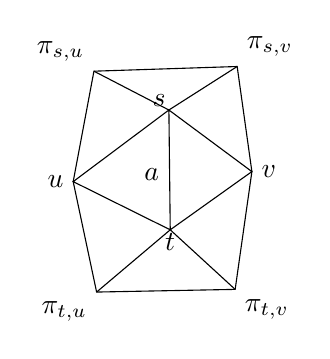
\begin{tikzpicture}[x=.85cm,y=.85cm]
\coordinate (lu) at (-1.12,1.65); \coordinate (ru) at (1.02,1.72);
\coordinate (u) at (-1.43,0); \coordinate (v) at (1.24,.15);
\coordinate (s) at (0,1.07); \coordinate (t) at (.02,-.72);
\coordinate (ld) at (-1.08,-1.65); \coordinate (rd) at (.99,-1.61);
\draw (lu)--(ru)--(v)--(rd)--(ld)--(u)--cycle;
\draw (lu)--(s)--(ru) (s)--(u)--(t)--(v)--(s)--(t) (ld)--(t)--(rd);
\node[above left] at (lu) {$\pi_{s,u}$}; \node[above right] at (ru) {$\pi_{s,v}$};
\node[left] at (u) {$u$}; \node[right] at (v) {$v$};
\node[above left,inner sep=1pt] at (s) {$s$}; \node[below,inner sep=1pt] at (t) {$t$};
\node[left] at (0,.1) {$a$}; \node[below left] at (ld) {$\pi_{t,u}$};
\node[below right] at (rd) {$\pi_{t,v}$};
\end{tikzpicture}}

Si on avait pris l'autre sommet $t$, on aurait trouvé l'arête $\{\deleted{\unsure{t_u}}\pi_{t,u},\deleted{\unsure{t_v}}\pi_{t,v}\}$ antipodique de $\{s_u,s_v\}$, d'où un unique élément $\rho_0(a)\in\bar A$. On trouve \inserted{ainsi} une application canonique
\[
 A\longrightarrow\bar A
\]
qui commute aux autom de $\Pi$, et en particulier à $\underline a$. Comme $\underline a$ opère trivialement sur $\bar A$, \deleted{\unsure{$\exists$}} $\rho_0$ se factorise en
\[
\bar A\longrightarrow\bar A
\]
On trouve
\[
\rho^2(\bar a)=\overline{\{u,v'\}}=\overline{\{v,u'\}}
\]
% archive sheet number: 18
\scanpage{20}
puis
\[
\rho^3(\bar a)=\bar a
\]
Donc
\[
\rho^3=\mathrm{id}_{\bar A}
\]
En particulier, $\rho$ est une \uline{permutation}. Toutes ses orbites sont de cardinal 3. Donc il y a cinq telles orbites.

Une orbite de $\rho$ s'appelle \uline{trièdre} \uline{distingué} \inserted{(de directions d'arêtes)} associé à $\rho$. Deux directions d'arêtes \inserted{$\alpha,\beta$} sont dites \uline{orthogonales} si elles sont \inserted{$\ne$ et} dans la $=$ orbite, \inserted{i.e.  \deleted{\unsure{arête}} $=$ trièdre distingué}, ce qui signifie aussi
\[
\beta=\rho\alpha\quad\text{ou}\quad\alpha=\rho\beta
\]
Pour tte \deleted{orthog} direction d'arête, il y a donc exactement deux directions d'arêtes orthogonales. [On notera que la relation d'orthogonalité est sym. par définition, mais la relation $\beta=\rho\alpha$ \deleted{\unsure{$\alpha$}} \inserted{entre $\alpha$ et $\beta$} ne l'est pas, évidemment.\unsure{]}

L'ens des trièdres distingués est un ens quotient de cardinal $5$ de $\bar A$, noté \deleted{\unsure{$T$} \unsure{$I$}} $T$. \inserted{\deleted{\unsure{$A$}} On a application canonique $\bar A\longrightarrow T$} On peut le considérer comme un ens quotient de $A$, formé de $5$ parties de cardinal $6$, chacune d'elles stable par $\underline a$.
% slanted
\margin{terminologie : arêtes orthogonales}

\deleted{\unsure{In}}Interprétation concrète en termes de coloriages,
% archive sheet number: 19
\scanpage{21}
\uline{Proposition} \deleted{\unsure{Pour tout|Remarque}} Deux arêtes orthogonales n'ont pas de sommet en commun.

En effet, les quatre arêtes orthogonales \unsure{à|:} $\{s,t\}$ sont $\{\pi_{s,u},\pi_{s,v}\}$, \deleted{et} $\{\pi_{t,u},\pi_{t,v}\}$ \deleted{et} d'une part, $\{u,v'\}$ et $\{v,u'\}$ d'autre part, elles ne rencontrent pas $\{s,t\}$

\uline{Corollaire} Pour tt $s\in S$, si $P(s)$ est l'ens des \deleted{\unsure{pts} $t\in S$ adjacents à $s$,} \inserted{arêtes incidentes à $s$}, l'application $a\mapsto\mathrm{tr}(\bar a)$ induit une bijection
\[
P(s)\longrightarrow T
\]
En effet, c'est une application injective entre deux ens de cardinal 5.

\uline{Corollaire} Soit $G_s^+$ le groupe des rotations de $\Pi$ fixant $s$ (i.e. les autom. fixant $s$, et induisant sur $\unsure{\mathscr P|P|\Phi}_{\geq s}$ une rotation \ldots) Alors \deleted{\unsure{$G_s^+$|$G_s$}} $T$ est un torseur sous $G_s^+$ -- donc si on fixe un gén. $u_s$ de $G_s^+$, $u_s$ est une permutation circulaire sur $T$

Comme $T$ est \inserted{de card} impair, on en conclut que $G_s^+$ opère par \uline{permutations paires}.

\uline{NB} Plus gén, on voit que les autom. d'un polygône combinatoire de rang \deleted{\unsure{impair sont des|impaire est dans}} $\equiv 1\ (4)$ (p.ex. d'un pentagône) induisent
% archive sheet number: 20
\scanpage{22}
\deleted{\unsure{par analog}} \inserted{des} permutations paires sur l'ens des sommets (ou, dualement, sur l'ens des côtés). \deleted{Donc} On en conclut que plus gén. $G_s$ opère \inserted{\unsure{fidèlt|fidèlem$^{\mathrm t}$|fidèlement}} sur $T$ par permutations paires. Aussi, on trouve que \deleted{pour} tt polygône combinatoire de rang $\deleted{\unsure{rg|n}}\equiv1\ (4)$, l'ens des sommets est canoniquement orienté, via épinglage qui permet de numéroter l'ens des sommets (et l'orientation de l'ens des sommets ne dépend pas de l'épinglage\ldots)

On peut \unsure{au|aussi|donc} dire que tt $s\in S$ définit sur $T$, via $P(s)\xrightarrow{\sim}T$, une structure polygonale (pentagonale) \inserted{$\pi_s$}, qui est invariante sous $G_s$ (qui opère exactement comme le groupe des automorphismes de $\pi_s$. A fortiori, $G_s$ invarie l'orientation correspondante de $T$, soit $\omega_s$, donc $G_s$ opère par permutations paires. [On verra plus bas que $\omega_s$ ne dépend pas en fait du choix de $s\in S$]

Fixons-nous un repère $r=\{s,a,f\}$ de $\Pi$, d'où des automorphismes $\sigma_0,\sigma_1,\sigma_2$ engendrant $G=\mathrm{Aut}(\Pi)$.
% archive sheet number: 21
\scanpage{23}
\figure{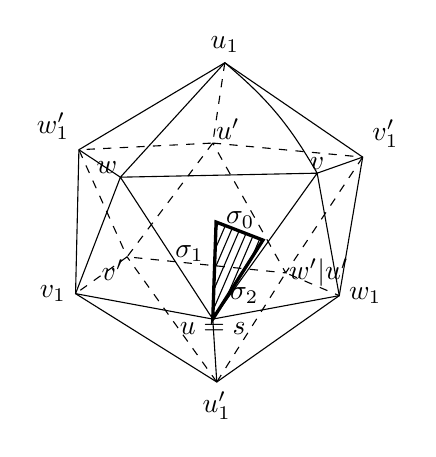
\begin{tikzpicture}[x=.85cm,y=.85cm]
\coordinate (ut) at (0,3); \coordinate (lt) at (-2.18,1.70); \coordinate (rt) at (2.06,1.59);
\coordinate (lb) at (-2.23,-.45); \coordinate (rb) at (1.71,-.48); \coordinate (bt) at (-.12,-1.77);
\coordinate (w) at (-1.56,1.29); \coordinate (v) at (1.38,1.35); \coordinate (u) at (-.18,-.83);
\coordinate (up) at (-.18,1.8); \coordinate (vp) at (-1.46,.10); \coordinate (wp) at (.91,-.14);
\draw (ut)--(lt)--(lb)--(bt)--(rb)--(rt)--cycle;
\draw[dashed] (up)--(vp)--(wp)--cycle (ut)--(up)--(lt)--(vp)--(lb)
 (bt)--(vp) (bt)--(wp)--(rb) (rt)--(wp) (up)--(rt);
\draw (w)--(v)--(u)--cycle (ut)--(w)--(lt) (lb)--(w) (lb)--(u)--(bt)
 (u)--(rb)--(v)--(rt) (ut) to[bend left=10] (v);
\coordinate (b) at (-.13,.62); \coordinate (c) at (.57,.35);
\begin{scope}\clip (u)--(b)--(c)--cycle;
\foreach \x in {-1.0,-.88,...,1.0}{\draw[thin] (\x,-.94)--++(.80,1.86);}
\end{scope}
\draw[very thick] (u)--(b)--(c)--cycle;
\node[above] at (ut) {$u_1$}; \node[above left] at (lt) {$w'_1$};
\node[above right] at (rt) {$v'_1$}; \node[left] at (lb) {$v_1$};
\node[right] at (rb) {$w_1$}; \node[below] at (bt) {$u'_1$};
\node[above left,inner sep=1pt] at (w) {$w$}; \node[above,inner sep=1pt] at (v) {$v$};
\node[below,inner sep=1pt] at (u) {$u=s$}; \node[above right,inner sep=1pt] at (up) {$u'$};
\node[below left,inner sep=1pt] at (vp) {$v'$}; \node[right,inner sep=1pt] at (wp) {$\unsure{w'|u'}$};
\node[above,inner sep=1pt] at (.23,.48) {$\sigma_0$}; \node[left] at (-.17,.15) {$\sigma_1$};
\node[right,inner sep=1pt] at (.03,-.48) {$\sigma_2$};
\end{tikzpicture}}

$\sigma_1$ et $\sigma_2$ fixent $s$, donc \deleted{conservent l'orientation de} \inserted{induisent des permutations} paires de $T$. D'autre part $\sigma_0$ conserve le troisième sommet $w$ (opposé à $a$) de la face (triangulaire) $f$, donc par ce qui précède \deleted{conserve} \inserted{induit} \unsure{égalt|ég\textsuperscript{t}} une orientation paire de $T$. Donc

\uline{Corollaire} $G=\mathrm{Aut}(\Pi)$ opère sur $T$ par permutations paires, i.e. on a
\[
G\longrightarrow\mathrm{Alt}_{T\deleted{\unsure{E}}}
\]
Comme $u\in G$, $s\in S$ implique évidemment
\[
\omega_{u(s)}=u(\omega_s)
\]
il s'ensuit, $G$ étant transitif sur $S$

\uline{Corollaire} Les orientations $\omega_s$ $(s\in S)$ de $T$ associées aux $s\in S$ sont ttes égales.

D'où une \uline{orientation} \uline{canonique sur} $T$ (évidemment conservée par $G=\mathrm{Aut}(\Pi)$).
% archive sheet number: 22
\scanpage{24}
\uline{Proposition} Considérons une face $f=\{u,v,w\}$. \deleted{Alors les trois arêtes} Soit $t_f=t$ l'ens des trois arêtes de $f$ (en correspondance $1$-$1$ avec l'ens de ses sommets), et soient $\{u_1,v_1,w_1\}$ les troisièmes sommets des \inserted{trois} faces \inserted{$\ne f$} adjacentes à ces arêtes. Alors

a) \deleted{\illegible{1}} $\rho$ induit la permutation circulaire \unsure{standart|standard} sur \unsure{tri-ens|les ens|les} \inserted{de} directions d'arêtes $\overline{\{u,v_1\}},\ \overline{\{v,w_1\}}\quad\overline{\{w,u_1\}}$ et sur l'ens des directions d'arêtes $\overline{\{u,w_1\}},\ \overline{\{w,v_1\}},\ \overline{\{v,u_1\}}$,
\margin{$u\,v\,w$\\$u\,w\,v$}
\deleted{et} \inserted{Considérons} les trièdres \inserted{dist.} associés à ces orbites de $\rho$, en corr. $1$-$1$ avec l'ens \inserted{$\{\omega,\omega'\}=\{\omega,\omega^{-1}\}$} des deux orientations (i.e des 2 ordres circulaires) sur $f$, soit $\{t_\omega,t_{\omega'}\}$

b) Les\deleted{\unsure{ens|trois}} trièdres distingués $\mathrm{tr}\,\overline{\{v,w\}}=t_u$, $\mathrm{tr}\,\overline{\{w,u\}}=t_v$, $\mathrm{tr}\,\overline{\{u,v\}}=t_w$, $t_\omega$ et $t_{\omega'}$ sont distincts.

\uline{Dém} a) est clair. \deleted{\unsure{Que|Pour}} $t_u,t_v,t_w$ soient distincts est un cas particulier de la prop. précédente, ainsi que $t_u\ne t_\omega=\mathrm{tr}\,\overline{\{w,u_1\}}$ $t_u\ne t_{\omega'}=\mathrm{tr}\,\overline{\{v,u_1\}}$ et de $=$ pour $t_v,t_w$.

\uline{Corollaire} On a une bijection canonique
\[
T\simeq f\amalg\mathrm{Or}(f)
\]
% archive sheet number: 23
\scanpage{25}
(où $f$ est identifié à un élément de $\unsure{\mathscr P|\mathfrak P}_3(S)$).

Cette bijection est évidemment compatible avec l'opération de $G_f\simeq D_3$ \inserted{$=\unsure{\mathfrak S|\mathscr S}_3$}, opérant sur \deleted{\unsure{$\mathbf Z/2$}} $\mathrm{Or}(f)$ via le quotient $\mathfrak S_2$ de $\mathfrak S_3$ (i.e. via signature) et sur $f$ \unsure{tautologique|tautologiqmt|tautologiquement}.

\deleted{Donc} [On retrouve que $G_f$ \deleted{conserve} \inserted{opère} par permutations paires sur $T$ --] On voit ainsi que \deleted{l'image de} $G_f$ \deleted{\unsure{dans $G$|dans}} \inserted{opère \unsure{fidèlt|fidèlement} sur $T$, et son image dans} $\mathfrak S_T$ (\deleted{\unsure{et est|contenue dans}} $\mathrm{Alt}_T$) est donc un ss-groupe d'ordre $6$. Donc l'image de $G$ dans $\mathrm{Alt}_T$ est d'ordre un multiple de $6$, et par les résultats \unsure{précédts|précédents} un multiple de $10$, donc un multiple de $30$.

\uline{Proposition} Soit $a\unsure{\in|=}\{s,t\}\in A$. Considérons \deleted{l'ens $\varphi$} les deux faces incidentes à $a$, et \inserted{l'ens $\varphi\in\mathscr P_2(S)$} leurs troisième\unsure{s} sommets $u,v$, \deleted{\unsure{Alors|dans $A$}} \deleted{de leurs arêtes} Considérons $a\times\varphi\longrightarrow A$ défini par $(s,u)\longmapsto\{s,u\}$. Alors les cinq éléments $\mathrm{tr}\,\overline{\{s,u\}}$ $(s\in a,u\unsure{\in|+}\varphi)$, $\mathrm{tr}\,\bar a$ de $T$ sont distincts.

Résulte des deux prop. précédentes.
% archive sheet number: 24
\scanpage{26}
On trouve ainsi une bijection canonique
\[
T\simeq\{\mathrm{tr}\,\bar a\}\amalg a\times\varphi,
\]
évidemment compatible avec l'action de $G_s\simeq\unsure{\mathfrak S|\mathscr S}_a\times\mathfrak S_\varphi\simeq\mathbb Z/2\mathbb Z\times\mathbb Z/2\mathbb Z$, qui opère donc \uline{fidèlement} sur $T$. On retrouve que $G_s$ opère sur $T$ par permutations paires, et \deleted{bref} de plus on conclut que l'image de $G$ dans $\mathrm{Alt}_T$ est d'ordre divisible par $4$. Étant déjà \inserted{d'ordre} divisible par $30$, il est divisible par $60$ Or $\mathrm{Alt}_T\deleted{\unsure{\{}}$ est d'ordre $60$, \deleted{on trouve} et \deleted{Aut} $G$ d'ordre $120$, on trouve

\uline{Th} L'hom canonique
\[
G=\mathrm{Aut}\underset{\substack{|\\\text{icos. comb}}}{\Pi}
 \longrightarrow\mathfrak S_{\underbrace{T(\Pi)}_{\substack{\text{ens des}\\\text{trièdres distingués}}}}
\]
a comme image $\mathrm{Alt}_T$, et comme noyau le ss-groupe \inserted{$\mathfrak z$} d'ordre $2$ engendré par l'antipodisme $\underline a$.

Comme \deleted{\illegible{1}} $\Pi$ \uline{est orientable} et $\underline a$ renverse \deleted{Corollaire} l'orientation, on trouve
\[
G\simeq \mathfrak z\times G^+
\]
donc
\[
G^+\xrightarrow{\sim}G/\mathfrak z
\]
donc
% archive sheet number: 25
\scanpage{27}
\uline{Corollaire}\qquad $G^+\xrightarrow{\sim}\mathrm{Alt}_T$

Reconstruction de l'icosaèdre \uline{orienté} par l'ens orienté $T$

Soit $\Pi$ icosaèdre, \deleted{\illegible{1}} pas orienté pour le moment. L'ens $T$ de ses trièdres distingués est orienté de façon canonique, soit $\unsure{\bar\omega|\varpi}$ son orientation. Sur $T\deleted{\unsure{\{}}$ il y a exactem$\unsure{^{\mathrm t}|t}$ $\frac12\,4!$ \inserted{$=12$} structures polygonales, qui se partagent en $2$ paquets de \inserted{$6$} structures polygonales associées à l'une et l'autre orientation. Soit $\mathrm{Pent}^+(T,\bar\omega)$ l'ens des \deleted{\unsure{$1$}}$6$ structures pentagonales associées à $\bar\omega$. On a une application canonique
\[
S/\deleted{\unsure{G}}\underline a\longrightarrow\mathrm{Pent}^+(T,\bar\omega)
\]
compatible avec op. de $G$. Or $G$ opère transitivement sur $S$, et il est immédiat que $\mathrm{Alt}_T$ opère transitivemt sur $\mathrm{Pent}^+(T,\bar\omega)$ (valable pour tt \unsure{$a$-|$n$-}polygône à $n\equiv1\ (4)$ côtés \ldots), donc l'application précédente est surjective, donc bijective
\[
S/\underline a\simeq\mathrm{Pent}^+(T,\bar\omega).
\]
% archive sheet number: 26
\scanpage{28}
Soit d'autre part
\[
\deleted{\unsure{A}}\ \mathbb A^{\unsure{'|\{}}(T)=
\left\{(t,\unsure{\pi|\Pi|\gamma},\bar a)\,\middle|\,
\begin{aligned}
&t\in T\\[-2pt]
&\pi\in\mathrm{Pol}(T\setminus\{t\})\\
&\bar a\in\mathrm{Ar}(\pi)/\mathrm{antipod}
\end{aligned}\right\}
\]
\inserted{$={}$Ens des $2$ diagonales du carré dual}

On voit que le cardinal de $\mathbb A'(T)$ est $5\cdot\frac12(4-1)!\cdot2=30$ \deleted{\unsure{$\times2=60$}}. Mais si $\alpha\in\mathbb A(T)$, $\alpha$ détermine une bijection
\[
T\simeq\{t\}\amalg a\times\varphi\qquad
(\text{où }\varphi=\mathrm{Ar}(\pi)\setminusa)
\]
d'où une orientation de $T$. Ainsi $\mathbb A(T)$ se décompose en $2$ paquets de $15$ éléments, associés aux deux orientations \inserted{$\unsure{\bar\omega|\varpi},-\bar\omega$} de $T$; on voit tout de suite que, sur chacun, telle $\mathbb A^+(T,\bar\omega)$, le groupe alterné $\mathrm{Alt}_T$ opère transitivemt. Ceci posé, on a une application canonique
\[
 A/\underline a\longrightarrow\mathbb A^+(T,\bar\omega),
\]
\inserted{compatible avec $G=\mathrm{Aut}(\Pi)$} et on voit comme précédemmt qu'elle est surjective, donc bijective.

Enfin, \unsure{on} a une application canonique
\[
 F/\underline a\longrightarrow\unsure{\mathscr P|\mathfrak P}_2(T)
\]
\figure{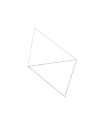
\begin{tikzpicture}[scale=.65,gray!45]
\draw[very thin] (0,0)--(.95,.13)--(.72,-.59)--cycle;
\draw[very thin,gray!25] (0,0)--(.13,.75)--(.95,.13);
\end{tikzpicture}}
compatible aux op. de $G$, donc (comme $\mathrm{Alt}_T$ est transitif sur $\mathscr P_2(T)$) surjective donc bijective.
% archive sheet number: 27
\scanpage{29}
Donc on a reconstruit les ens de sommets, d'arêtes, de faces de l'\uline{icosaèdre gauche} en termes de $(T,\unsure{\bar\omega|\varpi})$. Il faudrait reconstruire aussi les relations d'incidence.
\[
\begin{aligned}
\bar s\in\bar S&\longleftrightarrow\pi\in\mathrm{Pent}^+(T,\bar\omega)\\
\bar a\in\bar A&\longleftrightarrow\{\tau,\unsure{\gamma|\theta},\alpha\}\in\mathbb A^+(T,\bar\omega)\\
\bar f\in\bar F&\longleftrightarrow\deleted{\unsure{\{\omega,\omega'\}}}\ \Omega\in\unsure{\mathscr P|\mathfrak P}_2(T)
\end{aligned}
\]

\uline{Proposition}

a) $\bar s$ et $\bar a$ incidents sss $\gamma$ est la structure carrée sur $T\setminus\{\tau\}$ se déduisant de la structure pentagonale $\pi$ sur $T$ en prenant les sommets adjacents $u,v$ de $T$ à $t$, $\tilde u\ne\tau$ ($\tilde v\ne\tau$) adjacent à $u$, et la structure carrée de diagonales $\{u,\tilde u\},\{v,\tilde v\}$, donc \deleted{\unsure{$u\,v\,\tilde u\,\tilde v$}}
\diagram{\begin{tikzcd}[ampersand replacement=\&,row sep=small,column sep=small]
u\arrow[r,dash]\arrow[d,dash]\&v\\
\tilde v\arrow[r,dash]\&\tilde u
\end{tikzcd}}
, et $\alpha=\{\{u,v\},\{\tilde u,\tilde v\}\}$

\figure{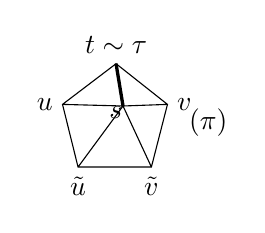
\begin{tikzpicture}[scale=.68]
\coordinate(t)at(0,1.1);\coordinate(u)at(-1,.34);\coordinate(v)at(.96,.34);
\coordinate(a)at(-.71,-.83);\coordinate(b)at(.66,-.83);\coordinate(s)at(.13,.31);
\draw (t)--(u)--(a)--(b)--(v)--cycle (u)--(s)--(v) (a)--(s)--(b);
\draw[very thick] (t)--(s);
\node[above]at(t){$t\sim\tau$};\node[left]at(u){$u$};\node[right]at(v){$v$};
\node[below]at(a){$\tilde u$};\node[below]at(b){$\tilde v$};
\node[below left,inner sep=0pt]at(s){$s$};\node[right]at(1.18,0){$(\pi)$};
\end{tikzpicture}}

\diagram{\begin{tikzcd}[ampersand replacement=\&,row sep=tiny,column sep=small]
\deleted{\unsure{\{s,u\}}}\arrow[r,dash]\&\deleted{\unsure{\{v,\tilde v\}}}\arrow[ddd,bend left]\\
\deleted{\{s,v\}}\arrow[r,leftrightarrow]\&\deleted{\{u,\tilde u\}}\\
\deleted{t}\&\deleted{\{t,u\}}\arrow[d,bend right,leftrightarrow]\\
\&\deleted{\{t,v\}}
\end{tikzcd}}

\diagram{\begin{tikzcd}[ampersand replacement=\&,row sep=tiny,column sep=small]
\{s,u\}\arrow[d]\&\\
\{s,v\}\arrow[d]\&\\
\{s,\tilde u\}\arrow[d]\&{\sim}\{t,v\}\\
\{s,\tilde v\}\arrow[uuu,bend left=48]\&{\sim}\{t,u\}
\end{tikzcd}}

[$\bar R=\vec A(\bar\Pi)$ s'identifie à l'ens des couples $(\pi,t)$, avec $\pi\in\mathrm{Pent}^+(T,\bar\omega)$, $t\in T$, donc $\bar R=\vec A(\bar\Pi)\simeq S(\bar\Pi)\times T\unsure{(\bar\Pi)}$

b) $\bar a$ et $\bar f$ sont incidents sss $\tau\in\underbrace{T\setminus\Omega}_{\unsure{\Phi''|\Phi}\deleted{\unsure{\varphi}}}$, \deleted{\unsure{$\mathrm{Alt}$}} $\gamma$ \inserted{sur $T\setminus\{\tau\}$} \deleted{\unsure{est défini}} par la condition que \inserted{$T\simeq\{\tau\}\amalg\bigl[\unsure{\Phi|\mathrm R}\setminus\{\tau\}\bigr]\amalg\Omega$}
\deleted{la relation ``ne pas être relié'' de}
\deleted{$\{T-\tau\}$ \unsure{est l'unique bijection|est l'unique bipartition} $\{\unsure{T|\Phi}-\tau\}$ et $\Omega$ telle que}
\deleted{\illegible{1}} 1°) $\unsure{\Phi|\mathrm R}-\tau$ et $\Omega$ sont des arêtes (opposées) \inserted{pour $\gamma$},
2°) et sont \deleted{\unsure{$\in$}} $\alpha$ (donc $\alpha$ est déterminé par $\gamma$ \unsure{l'est|l'étant}) \deleted{\unsure{et il y a a priori deux structures carrées possibles}}
\figure{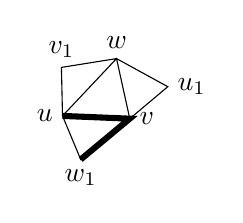
\begin{tikzpicture}[scale=.7]
\coordinate(a)at(-1,.88);\coordinate(w)at(0,1.04);\coordinate(b)at(.93,.53);
\coordinate(u)at(-.98,0);\coordinate(v)at(.24,-.05);\coordinate(c)at(-.65,-.79);
\draw (a)--(w)--(b)--(v)--(c)--(u)--cycle (u)--(w)--(v);
\draw[line width=2.2pt] (u)--(v)--(c);
\node[above]at(a){$v_1$};\node[above]at(w){$w$};\node[right]at(b){$u_1$};
\node[left]at(u){$u$};\node[right]at(v){$v$};\node[below]at(c){$w_1$};
\end{tikzpicture}}
\diagram{\begin{tikzcd}[ampersand replacement=\&,row sep=tiny]
\{u,w_1\}\arrow[d]\\
\{w_1,v\}\arrow[d]\\
\{v,w\}\arrow[d]\\
\{w,u\}\arrow[uuu,bend left=53]
\end{tikzcd}}
% archive sheet number: 28
\scanpage{30}
\uline{NB} Il y a a priori deux structures carrées sur $T\setminus\{\tau\}$ satisfaisant 1°), définies par les deux bijections possibles entre $\Phi\setminus\{\tau\}=\Omega'$ et $\Omega$ (relation de non-adjacence), mais on constate que les 2 \deleted{signatures} \inserted{orientations} de $T$ associées à ces deux choix de $\gamma$, lorsque $\alpha$ satisfait tjrs 2°), sont opposées, donc il y a exactemt un tel $\gamma$ tel que $(\tau,\gamma,\alpha)\in\mathbb A^+(T,\unsure{\bar\omega|\varpi})$ \ldots

\[
\bigl[\ R'=A^{\uparrow}(\bar\Pi)\simeq
\{(\Omega\unsure{'|^{\bullet}|\mbox{}},\Omega')\in\unsure{\mathscr P|\mathfrak P}_2(T)\times\mathscr P_2(T)\mid\Omega\cap\Omega'=\varnothing\}
\]

c) $\bar s$ et $\bar f$ sont incidents sss $\Omega$ est une \uline{\unsure{anticôte|anticôté}} pour la structure pentagonale $\pi$. [$R''\simeq{}$ ens des structures pentagonales sur $T$ munies d'une (anti) \unsure{côte|côté|arête} \inserted{au choix}]

\figure{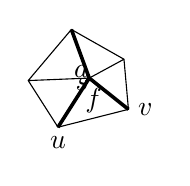
\begin{tikzpicture}[scale=.63]
\coordinate(a)at(-1,0);\coordinate(b)at(-.13,1.03);\coordinate(c)at(.93,.43);
\coordinate(d)at(1.02,-.58);\coordinate(e)at(-.40,-.94);\coordinate(s)at(.23,.05);
\draw(a)--(b)--(c)--(d)--(e)--cycle (a)--(s)--(c);
\draw[line width=1.3pt](b)--(s)--(e) (s)--(d);
\node[above left,inner sep=0pt] at (s){$a$};\node[below left,inner sep=0pt]at(s){$s$};
\node at (.32,-.40){$f$};\node[below]at(e){$u$};\node[right]at(d){$v$};
\end{tikzpicture}}
\margin{\uline{NB} $a\sim\{u,v\}$}

d) $\{\bar s,\bar a,\bar f\}$ forment un repère sss $\pi,(\tau,\gamma,\alpha)$ et $\Omega$ se déduisent de
$\{\underset{\inserted{\substack{\uparrow\\\mathrm{Pent}^+(T,\bar\omega)}}}{\pi},
\underset{\inserted{\substack{\uparrow\\T}}}{\tau},
\underset{\inserted{\substack{\uparrow\\\mathscr P_2(T)}}}{\Omega}\}$
satisfaisant $\tau\notin\Omega$, $\Omega$ anticôte pour $\pi$, $\tau$ adjacent \inserted{(pour $\pi$)} à un \uline{seul} sommet de $\Omega$
[ce qui donne, pour \deleted{\unsure{$\mathscr P_2$}} $\pi$ (6 choix) et $\Omega$ (5 \deleted{\unsure{et}} choix) choisis, 2 choix pour $\tau$], en prenant pour $\gamma$ l'unique structure de carré sur $T\setminus\{\tau\}$ pour laquelle $\Omega$, $\{u,v\}$ (ens des deux sommets adj. à $t$ \unsure{\}|)} et $\{\bar u,\bar v\}=T\setminus\{\tau\}-\{u,v\}$ sont des arêtes, et $\alpha=\{\{u,v\},\{\tilde u,\tilde v\}\}$ est le \unsure{contingent|côté-gauche|codiagonale} de $(T\setminus\{\tau\},\gamma\}$ qui ne contient pas $\Omega$. La donnée

\diagram{\begin{tikzcd}[ampersand replacement=\&,row sep=tiny,column sep=tiny]
\&\& A^{\vcenter{\hbox{\tikz[scale=.1]{\draw[->](0,0)--(0,1.5);\draw[->](0,0)--(1.5,0);}}}}\arrow[ddl]\arrow[d]\arrow[ddr]\&\&\\
\&\& A^{\wedge}\arrow[ddl]\arrow[ddr]\&\&\\
\&\vec A\arrow[dl]\arrow[dr]\&\& A^{\uparrow}\arrow[dl]\arrow[dr]\&\\
S\&\& A\&\& F
\end{tikzcd}}
\figure{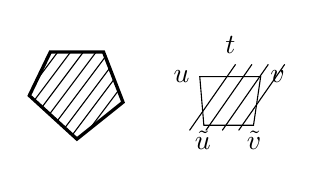
\begin{tikzpicture}[scale=.65]
\begin{scope}\clip (-.93,.05)--(-.52,.9)--(.52,.9)--(.9,-.08)--(0,-.8)--cycle;
\foreach \x in {-1.8,-1.55,...,1}{\draw (\x,-1)--++(1.5,2);}\end{scope}
\draw[very thick](-.93,.05)--(-.52,.9)--(.52,.9)--(.9,-.08)--(0,-.8)--cycle;
\begin{scope}[xshift=3cm]
\node at(0,1.03){$\deleted{\unsure{t}}$};\draw (-.6,.42)--(.59,.42)--(.45,-.53)--(-.52,-.53)--cycle;
\foreach \x in {-.8,-.48,-.16,.16}{\draw(\x,-.63)--++(.90,1.29);}
\node[left]at(-.61,.43){$\deleted{\unsure{u}}$};\node[right]at(.59,.42){$\deleted{\unsure{v}}$};
\node[below]at(-.54,-.46){$\deleted{\unsure{\tilde u}}$};\node[below]at(.46,-.46){$\deleted{\unsure{\tilde v}}$};
\end{scope}\end{tikzpicture}}
\figure{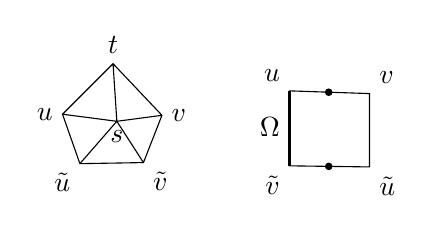
\begin{tikzpicture}[scale=.69]
\coordinate(t)at(0,1.2);\coordinate(u)at(-.93,.27);\coordinate(v)at(.90,.25);
\coordinate(x)at(-.61,-.64);\coordinate(y)at(.56,-.62);\coordinate(s)at(.07,.14);
\draw (u)--(t)--(v)--(y)--(x)--cycle (x)--(s)--(y) (u)--(s)--(v) (t)--(s);
\node[above]at(t){$t$};\node[left]at(u){$u$};\node[right]at(v){$v$};\node[below]at(s){$s$};
\node[below left]at(x){$\tilde u$};\node[below right]at(y){$\tilde v$};
\begin{scope}[xshift=4cm]
\draw(-.75,.7)--(.72,.65)--(.72,-.7)--(-.75,-.68)--cycle;
\draw[very thick](-.75,.7)--(-.75,-.68);
\fill (-.03,.675) circle(2pt) (-.03,-.69) circle(2pt);
\node[above left]at(-.75,.7){$u$};\node[above right]at(.72,.65){$v$};
\node[left]at(-.75,.04){$\Omega$};\node[below left]at(-.75,-.68){$\tilde v$};
\node[below right]at(.72,-.7){$\tilde u$};
\end{scope}\end{tikzpicture}}
% archive sheet number: 29
\scanpage{31}
du repère (défini par $\pi,\tau,\Omega$) définit un ordre sur $T$, car $\pi$ définit une structure pentagonale, $t_0=\tau$ une origine pour celle-ci, et désignant par $t_1=u$ l'unique $\in\Omega$ adjacent à $\tau$, on trouve un repère de \deleted{\unsure{$\mathscr P_2$}} $(T,\pi)$, d'où une énumération $T=\{t_0,t_1,t_2,t_3,t_4\}$, \inserted{qui est compatible avec l'orientation $\unsure{\bar\omega|\varpi}$.} Inversement, la donnée d'une telle énumération définit une structure pentagonale $\pi\in\mathrm{Pent}^{\unsure{+|2}}(T,\bar\omega)$, \deleted{un $\Omega=\{t_1,$} un $\tau=t_0\in T$, un $\Omega=\{t_1,t_3\}\in\unsure{\mathscr P|\mathfrak P}_2(T)$, définissant un élément de $\mathrm{Rep}(\bar\Pi)$ \ldots.

\figure{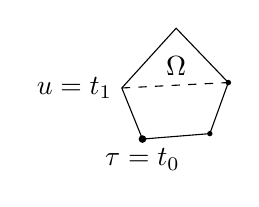
\begin{tikzpicture}[scale=.69]
\coordinate(u)at(-1,0);\coordinate(b)at(0,1.1);\coordinate(c)at(.96,.1);
\coordinate(d)at(.62,-.84);\coordinate(t)at(-.62,-.94);
\draw(u)--(b)--(c)--(d)--(t)--cycle;\draw[dashed](u)--(c);
\fill(t)circle(2pt) (c)circle(1.45pt) (d)circle(1.4pt);\node[left]at(u){$u=t_1$};\node[above]at(0,.05){$\Omega$};
\node[below]at(t){$\tau=t_0$};
\end{tikzpicture}}

Il reste à expliciter [pour $\Pi$ orienté]
\[
\left\{\begin{aligned}
\widetilde{S}(\bar\Pi)&\simeq S(\Pi)\\
\widetilde A(\bar\Pi)&\simeq A(\Pi)\\
\widetilde F(\bar\Pi)&\simeq F(\Pi)
\end{aligned}\right.
\]
en termes de $(T,\bar\omega)$. Et expliciter aussi, \deleted{\unsure{tant}} qu'à faire, la structure de $\bar\Pi$ comme polyèdre quotient \ldots.
% archive sheet number: 30
\scanpage{32}
\diagram{\begin{tikzcd}[ampersand replacement=\&,column sep=.48em,row sep=1.4em]
\& \& {D^{012}=A^{\vcenter{\hbox{\tikz[scale=.11]{\draw[->](0,0)--(0,1.4);\draw[->](0,0)--(1.6,0);}}}}}\arrow[dll]\arrow[dl]\arrow[d]\arrow[dr]\arrow[drr,very thick] \& \& \\
\widetilde S\arrow[d] \& {\substack{\vec A\\\shortparallel\\D^{01}}}\arrow[dl]\arrow[dr] \& \widetilde A\arrow[d] \& {\substack{A^\uparrow\\\shortparallel\\D^{12}}}\arrow[dl]\arrow[dr] \& \widetilde F\arrow[d]\\
{\substack{S\\ \shortparallel\\D^0}} \& \& {\substack{A\\ \shortparallel\\D^1}} \& \& {\substack{F\\ \shortparallel\\D^2}}
\end{tikzcd}\qquad
\begin{tikzcd}[ampersand replacement=\&,column sep=.35em,row sep=1.4em]
\& {A^{\vcenter{\hbox{\tikz[scale=.11]{\draw[->](0,0)--(0,1.4);\draw[->](0,0)--(1.6,0);}}}}=D^{012}}\arrow[d] \& \\
\& {\substack{A^\wedge\\\shortparallel\\D^{02}}}\arrow[dl]\arrow[dr] \& \\
{\substack{S\\ \shortparallel\\D^0}} \& \& {\substack{F\\ \shortparallel\\D^2}}
\end{tikzcd}}

Icosaèdre gauche (sommets $S$ etc\ldots) en termes de $(E,\omega)$, $E$ ens \unsure{à|:} $5$ éléments, $\omega$ une orientation

\diagram{$\begin{array}{ll}
S\simeq\mathrm{Pent}_\omega(E)&\text{struct. pent. comp. avec }\omega\\
A\simeq\deleted{\unsure{\mathscr P}}\mathrm{Car}(E)&\shortstack[l]{partitions de degrés $(2,2,1)$\\$\simeq$ structures carrées sur une partie de $E$}\\
F\simeq\deleted{\unsure{\mathscr P_3|\mathfrak P_3}}\mathrm{Tr}_3(E)&\shortstack[l]{\deleted{parties à $3$ él.}\\triangles $\subset E$}\\
\vec A\simeq\mathrm{Pent}^s_\omega(E)&\shortstack[l]{$\omega$-structures pentagonales à somm.\\marqué}\\
A^\uparrow\simeq\deleted{\unsure{\mathscr P_3|\mathfrak P_3}}\unsure{\dot{\mathrm{Tr}}_3|\mathrm{Tr}_3}(E)&\text{\deleted{parties à trois él.} \inserted{triangles} ponctués}\\
A^\wedge\simeq\mathrm{Pent}^a_\omega(E)&\text{structure pent. à arête marquée}\\
\hfill\shortparallel\hfill&\\[-3pt]
\hfill\mathrm{Pent}^s_\omega(E)\hfill&\\
A^{\vcenter{\hbox{\tikz[scale=.11]{\draw[->](0,0)--(0,1.4);\draw[->](0,0)--(1.6,0);}}}}\simeq\mathrm{Rep}_\omega(E)&\shortstack[l]{ordres totaux\\sur $E$ comp.\\avec $\omega$}
\end{array}$}

\figure{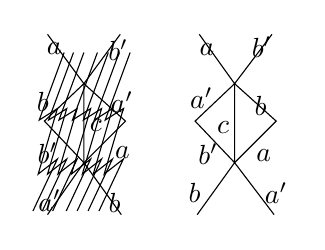
\begin{tikzpicture}[scale=.66,baseline]
\draw(-.7,1.85)--(0,.9)--(.8,.18)--(0,-.62)--(-.76,.18)--(0,.9)--(.7,1.85);
\draw(0,.9)--(0,-.62)--(-.7,-1.62) (0,-.62)--(.72,-1.62);
\node at(-.57,1.57){$\deleted{a}$};\node at(.66,1.55){$\deleted{b'}$};
\node at(-.79,.54){$\deleted{b}$};\node at(.73,.55){$\deleted{a'}$};
\node at(.23,.1){$\deleted{c}$};\node at(-.70,-.43){$\deleted{b'}$};\node at(.74,-.43){$\deleted{a}$};
\node at(-.66,-1.35){$\deleted{a'}$};\node at(.59,-1.39){$\deleted{b}$};
\foreach \x in {-.76,-.58,-.38,-.12,.09,.30,.51}{\draw[thin](\x-.22,-1.55)--(\x+.25,-.55)--(\x-.12,-.84)--(\x+.25,.42)--(\x-.1,.2)--(\x+.38,1.5);}
\begin{scope}[xshift=2.9cm]
\draw(-.68,1.85)--(0,.9)--(.8,.18)--(0,-.62)--(-.76,.18)--(0,.9)--(.72,1.85);
\draw(0,.9)--(0,-.62)--(-.72,-1.62) (0,-.62)--(.76,-1.62);
\node at(-.53,1.56){$a$};\node at(.52,1.60){$b'$};\node at(-.64,.62){$a'$};\node at(.5,.48){$b$};
\node at(-.22,.06){$c$};\node at(-.51,-.45){$b'$};\node at(.56,-.49){$a$};\node at(-.77,-1.21){$b$};\node at(.8,-1.21){$a'$};
\end{scope}
\end{tikzpicture}}

\figure{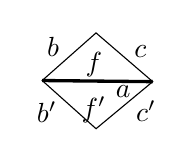
\begin{tikzpicture}[scale=.72]
\draw(-.95,.12)--(0,.96)--(1,.10)--(0,-.73)--cycle;
\draw[very thick](-.95,.12)--(1,.10);
\node at(-.76,.72){$b$};\node at(.78,.64){$c$};\node at(-.04,.40){$f$};\node at(.48,-.08){$a$};
\node at(-.04,-.40){$f'$};\node at(-.87,-.43){$b'$};\node at(.88,-.42){$c'$};
\end{tikzpicture}\qquad
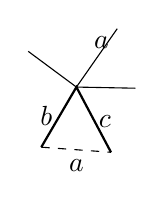
\begin{tikzpicture}[scale=.72]
\draw(-.85,.95)--(0,.32)--(.72,1.35) (0,.32)--(1.04,.30);
\draw[thick](-.62,-.74)--(0,.32)--(.61,-.83);\draw[dashed](-.62,-.74)--(.61,-.83);
\node at(.44,1.10){$a$};\node at(-.53,-.19){$b$};\node at(.50,-.28){$c$};\node[below]at(0,-.79){$a$};
\end{tikzpicture}}

\diagram{$\begin{array}{ll}
\widetilde S\simeq\deleted{\unsure{\mathrm{Pent}_\omega(E)}}\overrightarrow{\mathrm{Pent}}_\omega(E)&\shortstack[l]{permutations circulaires comp.\\avec $\omega$}\\
\widetilde A\simeq\overrightarrow{\mathrm{Car}}(E)&\text{carrés orientés }\subset E\\
\widetilde F\simeq\deleted{\unsure{\mathscr P_3|\mathfrak P_3}}\overrightarrow{\mathrm{Tr}}_3(E)&\shortstack[l]{triangles orientés $\subset E$\\\deleted{parties à trois él. avec ordre circ. dessus}}
\end{array}$}

\[
\left\{\begin{aligned}
\sigma_0(a_1,\underline{a_2,a_3,a_4,a_5})&=(a_1,a_4,a_5,a_2,a_3)\\
\sigma_1(a_1,a_2,a_3,a_4,a_5)&=(a_2,a_1,a_5,a_4,a_3)\\
\sigma_2(a_1,a_2,a_3,a_4,a_5)&=(a_1,a_5,a_4,a_3,a_2)
\end{aligned}\right.
\]
\figure{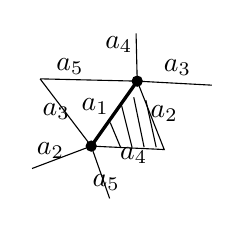
\begin{tikzpicture}[scale=.73]
\coordinate(p)at(-.56,-.37);\coordinate(q)at(.24,.76);\coordinate(r)at(.71,-.43);\coordinate(l)at(-1.45,.80);
\draw(l)--(q)--(1.54,.69) (q)--(.22,1.59) (l)--(p)--(r)--(q) (-1.59,-.76)--(p)--(-.24,-1.28);
\draw[very thick](p)--(q);\fill(p)circle(2.8pt) (q)circle(2.8pt);
\foreach \x/\y in {-.23/.04,-.03/.33,.18/.48,.39/.43}{\draw[thin](\x,\y)--(\x+.18,-.39);}
\node at(-.49,.32){$a_1$};\node at(.71,.20){$a_2$};\node at(.18,-.54){$a_4$};
\node at(-1.17,.23){$a_3$};\node at(-1.27,-.44){$a_2$};\node at(-.30,-1.01){$a_5$};
\node at(-.93,1.02){$a_5$};\node at(-.08,1.39){$a_4$};\node at(.94,1.00){$a_3$};
\end{tikzpicture}}
% archive sheet number: 31
\scanpage{33}
\[
\begin{aligned}
\rho_f=\sigma_1\sigma_0&:\quad(a_1,a_2,a_3,a_4,a_5)\unsure{\longmapsto|\mathrel{\vdash\!\!\!-\!\!\bullet}}(a_4,a_1,a_3,a_2,a_5)\\
\rho_s=\sigma_2\sigma_1&:\quad(a_1,a_2,a_3,a_4,a_5)\longmapsto(a_2,a_3,a_4,a_5,a_1)\\
\sigma=\sigma_0\sigma_1&:\quad(a_1,a_2,a_3,a_4,a_5)\longmapsto(a_1,a_3,a_2,a_5,a_4)
\end{aligned}
\]
% archive sheet number: 32
